%% Genatic Algorthims introduction
\subsection{GA Introduction}
\begin{frame}{Genetic Algorithms}
A search technique mimicking natural evolution.
\begin{columns}[onlytextwidth]
\begin{column}{0.45\textwidth}
\small
\begin{itemize}
	\item Population of candidate solutions is evolved toward better solutions
	\item Each candidate has properties that can be mutated and altered
	\item Traditionally solutions are represented as bit strings or trees
\end{itemize}
\end{column}
\begin{column}{0.45\textwidth}
	\centering
	\begin{figure}
		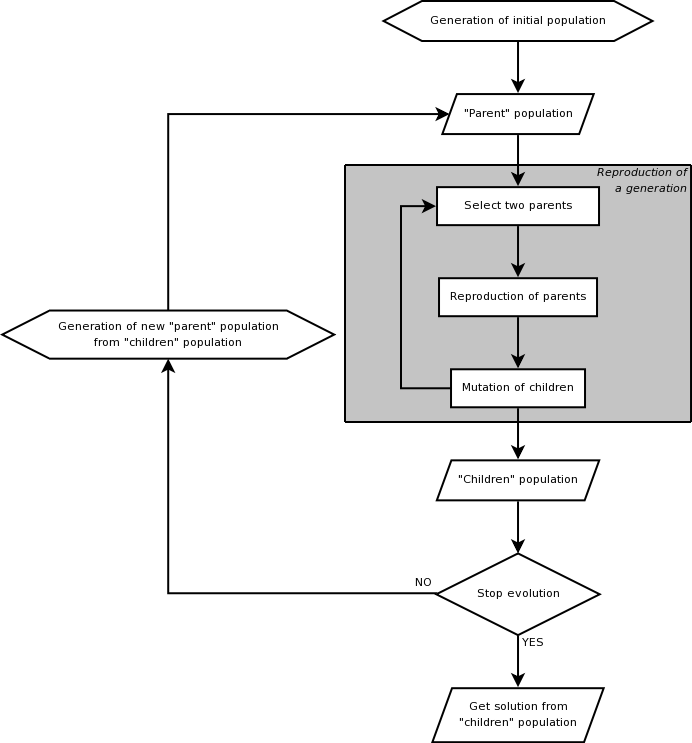
\includegraphics[width=\textwidth]{genetic_algorithm_principle}
	\end{figure}
\end{column}
\end{columns}
\end{frame}
\begin{frame}{Crossover Operations}
	\begin{columns}[onlytextwidth]
	\begin{column}{0.4\textwidth}
  \begin{itemize}
    \item Single point - choose a single point (two segments) to crossover
    \item Two point - choose two points (three segments) to crossover
    \item Uniform - Uniformly cross over based on some probability
  \end{itemize}
	\end{column}
	\begin{column}{0.55\textwidth}
    \begin{figure}
      \centering
      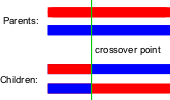
\includegraphics[width=0.3\textwidth]{SinglePointCrossover.png}
    \end{figure}
    \begin{figure}
      \centering
      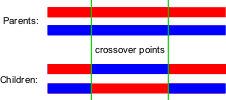
\includegraphics[width=0.3\textwidth]{TwoPointCrossover.png}
    \end{figure}
    \begin{figure}
      \centering
      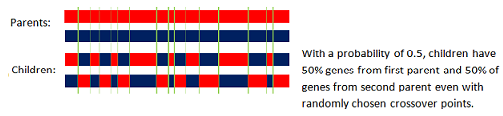
\includegraphics[width=\textwidth]{UniformCrossover.png}
    \end{figure}
	\end{column}
	\end{columns}
\end{frame}
\begin{frame}{Mutation Operations}
Mutations are designed to avoid local minima
\begin{columns}
\begin{column}{0.45\textwidth}
  \begin{itemize}
    \item Swap
    \item Flip - flips (inverts) all of the bits
  \end{itemize}
    \begin{figure}
      \centering
      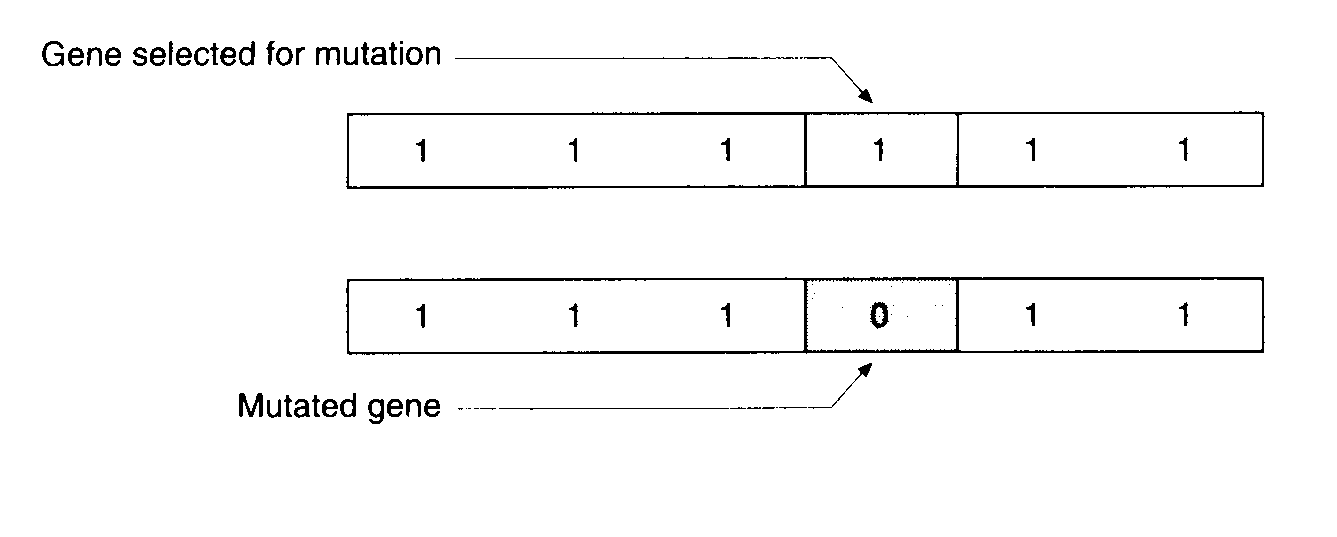
\includegraphics[width=0.4\textheight]{mutation_example.png}
    \end{figure}
	Typically set to be around a few percent
\end{column}
\begin{column}{0.45\textwidth}
\begin{figure}
	\centering
	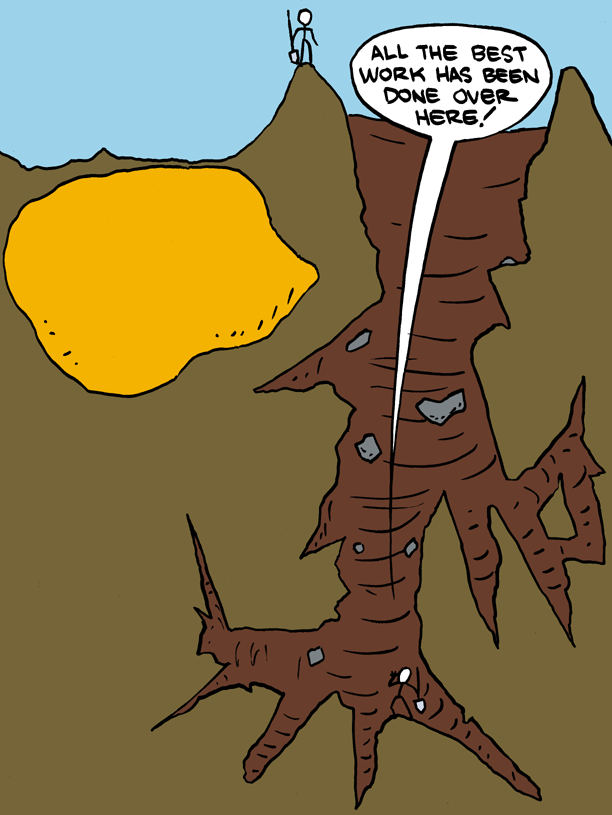
\includegraphics[width=0.75\textwidth]{AllTheBestWork.png}
\end{figure}

\end{column}
\end{columns}
\end{frame}
